\label{chp:dynamics}
In the previous chapter, we have seen how the many-body problem can be decoupled into an electronic problem %given by Eq.\,\eqref{eq:Hsolution1}, 
which can be solved in the framework of DFT, and a nuclear problem %given by Eq.\,\eqref{eq:chi2} 
that describes the dynamical properties of the nuclei. This was achieved by means of the Born-Oppenheimer approximation where electron-nucleus interactions beyond a parametric dependence on each other are neglected~\cite{BornOppenheimer}.
% \mscomment{dynamics are decoupled}

\newthought{We will now approach} the description of the nuclear dynamics from two sides: First, we introduce the \emph{harmonic approximation} in which the nuclear Schr\"odinger equation is solved for an approximated potential in terms of vibrational eigenmodes. We will discuss extended systems next, in particular crystalline systems with long-range order.
Second, we treat the nuclei as \emph{classical} particles on the full, non-truncated Born-Oppenheimer potential $E^{\rm BO} ({\bf R})$. This will lead to the formulation of \emph{ab initio molecular dynamics} (aiMD). In a last step, we will connect the two approaches to allow for extracting phonon properties from MD simulations.
As no electron will appear anymore, $N \equiv N_{\rm Nuc}$ will henceforth denote the number of nuclei in the system of interest, and we denote the Born-Oppenheimer potential simply as \emph{the} potential, 
$$E^{\rm BO} ({\bf R}) \equiv \mathcal V ({\bf R})~.$$

\newthought{To set the stage, we recall the Schr\"odinger equation} for the nuclear wavefunction $\chi ({\bf R})$ corresponding to the electronic ground state as initially defined in Eq.\,\eqref{eq:chi2},
\begin{align}
\left( \mathcal T + \mathcal V ({\bf R}) - E \right) \chi ({\bf R})
= 0~,
\label{eq:BOSE}
\end{align}
where
\begin{align}
\mathcal  T
= \sum_I \frac{- \hbar^2}{2 M_I} \frac{\partial^2}{\partial {\bf R}_I^2}~,
\label{eq:Tnuc2}
\end{align}
is the nuclear kinetic-energy operator as before.


\section{Harmonic Approximation}
\label{sec:HA}
The Born-Oppenheimer potential $\mathcal V ({\bf R})$ in Eq.\,\eqref{eq:BOSE} is an ordinary function of the\marginnote{Remember $N \equiv N_{\rm Nuc}$.} $3 N$ coordinates ${\bf R} = ({\bf R}_1, \ldots, {\bf R}_{N})$ and therefore can be expanded as a Taylor series in displacements ${\bf U} \equiv \Delta {\bf R}$ about a given configuration ${\bf R}^0$,~i.\,e.,
\begin{align}
\begin{split}
  \mathcal V ({\bf R} = {\bf R}^0 + {\bf U})
    = \mathcal V ({\bf R}^0)
    &+ \sum_{I, \alpha} 
      \left. \frac{\partial \mathcal V({\bf R})}{\partial R^\alpha_I} 
      \right\vert_{{\bf R}^0}
    \,U^\alpha_I
    \\
    &
    + \frac{1}{2}
    \sum_{\substack{I, J \\ \alpha, \beta}}
    \left.\frac{\partial^{2} \mathcal{V}(\mathbf{R})}{\partial R_{I}^{\alpha} \partial R_{J}^{\beta}}\right|_{\mathbf{R}^{0}}
    \, U_I^\alpha U_J^\beta
    \\
    &+\frac{1}{3!}\cdots ~,
\end{split}
\end{align}
where the expansion coefficients are called \emph{force constants}. In particular, we have the \emph{harmonic force constants}
\begin{align}
  % \Phi_{\alpha, \beta}^{I, J}
  \Phi_{I \alpha, J \beta}
  \equiv \left.\frac{\partial^{2} \mathcal{V}(\mathbf{R})}{\partial R_{I}^{\alpha} \partial R_{J}^{\beta}}\right|_{\mathbf{R}^{0}}~.
  \label{eq:FC2}
\end{align}
The harmonic approximation is typically used to assess dynamical properties of a system in some confined phase-space region close to a (local) minimum of the potential-energy surface.\footnote{See section \ref{sec:ltrm} in the appendix for details on geometry optimization in the context of crystal lattices.} A local minimum configuration ${\bf R}^0$ is characterized by
\begin{align}
	\left. \frac{\partial V({\bf R})}{\partial R^\alpha_I} 
	\right\vert_{{\bf R}^0} 
		&~=~ 0 \quad\text{for all}\quad (I, \alpha),~\text{and} \\
	\sum_{\substack{I, J \\ \alpha, \beta}}
	% \Phi_{\alpha, \beta}^{I, J}
	\Phi_{I \alpha, J \beta}
	\, U_I^\alpha U_J^\beta
		&~>~ 0 \quad\text{for all possible}\quad \set{{\bf U}_I}~.
	\label{eq:ha.positive}
\end{align}
The condition in Eq.\,\eqref{eq:ha.positive} is satisfied when the harmonic force constants $\Phi_{I \alpha, J \beta}$ are positive-definite. It needs to be fulfilled to make the Hamiltonian bounded. Details on how to obtain force constants numerically are given in appendix~\ref{app:force_constants}.

\newthought{We define \emph{mass-reduced coordinates}} for the displacements,
\begin{align}
	{\bf u}_I 
		&\equiv \sqrt{M_I} {\bf U}_I~, 
		\label{eq:uI} \\
	{\bf p}_I 
		&\equiv -\im \hbar \frac{\partial}{\partial {\bf u}_I}~,
		\label{eq:pI} \\
	% D_{\alpha, \beta}^{I, J}
	D_{I \alpha, J \beta}
		&\equiv \frac{1}{\sqrt{M_I M_J}} 
		%\Phi_{\alpha, \beta}^{I, J}
		\Phi_{I \alpha, J \beta}~,
		\label{eq:D}
\end{align}
where Eq.\,\eqref{eq:D} defines the \emph{dynamical matrix} $\rm D$.\footnote{There seems to be no general agreement that the matrix $\rm D$,~i.\,e.,~the mass-weighted force constants, are called ``dynamical matrix'', or if this term is reserved for the Fourier transformed matrices studied in periodic systems. However, we follow Born and Huang in using the term dynamical matrix irrespective of the question of lattice periodicity~\cite[p.\,173]{BornHuang}.}
Expressed in the mass-reduced coordinates ${\bf u} = \set{{\bf u}_I}$ and ${\bf p} = \set{{\bf p}_I}$, the harmonic Hamiltonian reads
\begin{align}
	\begin{split}
		\mathcal{H}^{(2)}({\bf p}, {\bf u})
			&= \mathcal T ({\bf p}) + \mathcal{V}^{(2)} ({\bf u})\\
			&= \halb \sum_I {\bf p}_I^2 + 
				\halb \sum_{\substack{I, J \\ \alpha, \beta}}
					D_{I \alpha, J \beta}
					\, u_I^\alpha u_J^\beta~.
	\end{split}
	\label{eq:ha.H1}
\end{align}
%
As required in Eq.\,\eqref{eq:ha.positive}, the dynamical matrix $\rm D$ needs to be positive definite to make $\mathcal H^{(2)}$ bounded. Furthermore, we see from Eq.\,\eqref{eq:FC2} that $\rm D$ is symmetric in the $3N$ coordinates $(I, \alpha)$ by the differentiability of the underlying potential $\mathcal V ({\bf R})$,
\begin{align}
	D_{I \alpha, J \beta} = D_{J \beta, I \alpha}~.
	\label{eq:D.symmetric}
\end{align}
The eigenvalues of $\rm D$ will therefore be real and positive, and the eigenvectors will be real and orthogonal. We denote the eigensolutions as \emph{modes} labeled by $s$, with eigenvalues $\omega_s^2$, and the normalized eigenvectors are ${\bf e}_s = \set{{\bf e}_{s, I}}$. The dynamical matrix elements can be rewritten in therms of the eigenvectors and eigenvalues as
\begin{align}
%	\sum_{J \beta}
%		D_{I \alpha, J \beta} \, e_{s, J \beta} 
%			&= \omega^2_s \, e_{s, I \alpha}~,~\text{or} 
%			\label{eq:sum_D_IJ} \\
		D_{I \alpha, J \beta}
			&= \sum_s \omega^2_s \, e_{s, I \alpha} e_{s, J \beta}~,
			\label{eq:D_IJ}
\end{align}
and the eigenvectors fulfill
\begin{align}
	\sum_{I \alpha} e_{s, I \alpha} e_{s', I \alpha} = \delta_{s s'}
	\quad \text{and} \quad
	\sum_{s} e_{s, I \alpha} e_{s, J \beta} = \delta_{IJ} \delta_{\alpha \beta}~.
	\label{eq:completeness.e_s}
\end{align}
Using the dynamical matrix elements expressed in terms of eigenvectors and eigenvalues,~Eq.\,\eqref{eq:D_IJ}, the harmonic Hamiltonian as defined in Eq.\,\eqref{eq:ha.H1} can be rewritten as
\begin{align}
	\mathcal{H}^{(2)}({\bf p},  {\bf u})
		&= \halb \sum_s p_s^2 + 
		\halb \sum_{s} \omega_s^2	\, u_s^2~.
\label{eq:ha.H2}
\end{align}
Here, we implicitly defined the $3N$ \emph{normal coordinates} $u_s$ and their conjugate momenta $p_s$ via the orthogonal transformation\footnote{Using vector notation $${\bf e}_{s, I} \cdot {\bf u}_I = \sum_{\alpha} e_{s, I \alpha} u_I^\alpha~.$$}
\begin{align}
	u_s
		&= \sum_{I} {\bf e}_{s, I} \cdot {\bf u}_{I}~,\quad\text{and}
		\label{eq:u_s} \\
%	p_s
%		&= -\im \hbar \frac{\partial}{\partial u_s}~.
%	\\
	p_s
	&=\sum_{I} {\bf e}_{s, I} \cdot {\bf p}_{I} ~.
		\label{eq:p_s}
\end{align}
The Hamiltonian expressed in terms of the normal coordinates, Eq.\,\eqref{eq:ha.H2}, contains no cross-terms between different modes $s$ and $s'$. Rewritten in terms of this Hamiltonian, the wave equation \eqref{eq:BOSE} reads
\begin{align}
	\left\{
		\halb \sum_s p_s^2 + \halb \sum_{s} \omega_s^2	\, u_s^2 - E~.
	\right\} \chi ({\bf u})
	= 0
	\label{eq:ha.SE.2}
\end{align}
Since the Hamiltonian is a sum of terms, each depending on one coordinate only, the total bosonic nuclear wavefuntion $\chi$ can be separated into a product of wavefunctions for each mode~\cite[p.\,175]{BornHuang},
\begin{align}
	\chi({\bf u}) = \prod_{s} \chi_s (u_s)~.
	\label{eq:ha.chi}
\end{align}
We end up with a set of $3N$ uncoupled equations, one for each mode $s$:
\begin{align}
	\left\{	\halb \left( p_s^2 + \omega_s u_s^2 \right)	- E_s	\right\} \chi_s (u_s)
		= 0~,
	\label{eq:ha.SE.single}
\end{align}
where the total energy of the nuclei is the sum of each mode contribution $E = \sum_s E_s$. Equation \eqref{eq:ha.SE.single} is the familiar equation for a harmonic oscillator of frequency $\omega_s$~\cite{Dirac1981}, thereby establishing $\omega_s$ as the \emph{eigenfrequency} of the mode $s$. Permissible solutions are labeled by the integer $n_s \in \mathds N_0$ and the eigenvalue $E_s$ depends on $n_s$ via
\begin{align}
	E_s(n_s) = \hbar \omega_s \left( n_s + \halb \right)~.
	\label{eq:E_s}
\end{align}
The state of the entire system is therefore specified by the $3N$ quantum numbers ${\bf n} = (n_1, \ldots, n_{3N})$, and the total energy of the system is
\begin{align}
	E ({\bf n}) = \sum_s \hbar \omega_s \left( n_s + \halb \right)~.
\end{align}
This derivation is generally valid for a system of $N$ particles described by a potential-energy surface of which a (local) minimum ${\bf R}^0$, and the matrix of second derivatives at this configuration, $\Phi_{IJ}$, is known. The thermodynamic properties of such a system of harmonic oscillators follow from this spectrum in straighforward fashion~\cite{BornHuang}.


\section{Extended Systems}
\label{sec:extended_systems}
\REM{Move up, include discussion of symmetry beyond translational}
The expressions presented in the previous section are generally valid for a system of $N$ nuclei. Macroscopic materials, however, consist of $\sim 10^{23}$ atoms. From a microscopic point of view, this number is virtually infinite, and mathematically described by the \emph{bulk limit} $N \to \infty$. The most common way to deal with this bulk limit is to impose \emph{periodic boundary conditions} on a finite region of space,~i.\,e.,~a \emph{generating volume}, and normalize the quantities of interest to this volume~\cite{BornHuang}. This procedure can be adopted for extended system such as liquids, amorphous solids such as glasses, and crystals. Since we are interested in the special case of crystals with an inherent periodic long-range order throughout this work, it is beneficial to first introduce the concept of a \emph{crystal lattice} that describes a bulk crystal in terms of a \emph{unit cell} arranged periodically in three dimensional space~\cite{Sands1969}. The periodic boundary conditions are then imposed on a generating volume containing several unit cells,~i.\,e.,~a \emph{supercell}.

\subsection{Periodic systems: Crystals}
% As already mentioned in Sec.~\ref{sec:theory.periodic.1},
%\newthought
{The crystalline state is characterized by a periodic long-range order of the potential energy $\mathcal V ({\bf R})$}. We describe this order in terms of the \emph{Bravais vectors} 
\begin{align}
	{\bf L} = L^\mu {\bf a}_\mu \quad\text{with}\quad L^\mu \in \mathds Z,
	\label{eq:L_Bravais}
\end{align}
where $\set{{\bf a}_\mu}$ are \emph{lattice vectors} spanning the unit cell of the %crystal, and $L^\mu$ are integers.
crystal.\footnote{Notation: We index components in the crystal basis $\set{{\bf a}_\mu}$ with $\mu, \nu$, as opposed to Cartesian components indexed by $\alpha, \beta~.$ Summing convention is implied as explained in appendix~\ref{app:notation}.} The Bravais vectors $\bf L$ span a regular grid,~i.\,e.,~a \emph{lattice}, and are therefore also called \emph{lattice points}.

\newthought{The invariance of the potential energy under translations by arbitrary Bravais vectors} $\bf L$ is defined as follows:
Let ${\bf R} = \set{{\bf R}_I}$ be a configuration of atoms, %in a local minimum of the potential energy, 
and let ${\bf R}^{\prime} = \set{{\bf R}^{\prime}_{I}}$ denote the configuration obtained by moving all atoms by a Bravais vector ${\bf L}$,
\begin{align}
	{\bf R}^{\prime}_{I} = \fD {\bf R}_{I} + {\bf L}~,
	\label{eq:RI'}
\end{align}
%
then for each configuration ${\bf R}$, ${\bf R}'$, the potential energy is unchanged,
\begin{align}
%	{\bf R}^{0 \prime}
%	= \set{{\bf R}_{I'}^0 }
%	&= {\bf R}^0 = \set{{\bf R}_{I}^0 }~,
%	\quad\text{and}
%	\label{eq:inv.R0} \\
	\mathcal{V} \left( {\bf R}' = \set{{\bf R}_{I} + {\bf L}} \right)
	&= \mathcal{V}({\bf R} = \set{{\bf R}_{I}} ) 
	\quad\text{for all}\quad {\bf L} = L^\mu {\bf a}_\mu~.
	% \quad\text{with}\quad \set{L^\mu \in \mathds{N}_0}
	\label{eq:inv.V}
\end{align}
%
As a consequence of this translational invariance, we observe that the reference configurations ${\bf R}^{0} = \set{{\bf R}^{0}_{I}}$ of the potential both before and after translating the system by $\bf L$ are unchanged,\footnote{Reference positions are typically thermodynamic expectation values of the atomic positions. In simple systems, these coincide with local minima of the potential.} \emph{and} there is a bijective permutation map $P_{\bf L}$ between the atomic positions ${\bf R}^{0 \prime}_{I}$ and ${\bf R}^{0}_{I'}$ which fulfills
\begin{align}
	P_{\bf L} : I \to I' \quad\text{such that}\quad
	{\bf R}^{0 \prime}_{I}
		= {\bf R}^{0}_{I'}~.
	\label{eq:translation.permutation}
\end{align}
This statement is equivalent to requiring that the configurations ${\bf R}^{0 \prime}_{I}$ and ${\bf R}^{0}_{I}$ are indistinguishable.\footnote{This requirement is obviously not fulfilled for molecules, where rigidly shifting all atoms can by no means induce a permutation map between atoms.} 
Writing the atomic configurations as reference positions plus displacements, ${\bf R} = {\bf R}^0 + {\bf U}$, this corresponds to a permutation of the displacements of the atoms, $U_I \to U_{I'}$ according to $P_{\bf L}$ defined in Eq.\,\eqref{eq:translation.permutation}. Figure\,\ref{fig:translation.permutation} shows a one-dimensional depiction of the relation between discrete translation by Bravais vectors and the permutation map.
\begin{marginfigure}
	\centering
	% \includegraphics[width=.68\textwidth]{./sketches/permutation1.jpg}
	\includegraphics[width=\textwidth]{./data/sketches/permutation1.jpg}
	\caption{A linear chain with three atoms (bullets) displaced from their equilibrium position (open circels). With periodic boundary conditions, the consecutive translation by a lattice vector $a$ induces a permutation of the atoms,~i.\,e.,~$(1, 2 , 3) \to (3, 1, 2) \to (2, 3, 1)$.}
	\label{fig:translation.permutation}
\end{marginfigure}

We can draw important conclusions from Eq.\,\eqref{eq:translation.permutation} and \eqref{eq:inv.V}. First, the existence of the map $P_{\bf L}$ enables us to write every atomic coordinate ${\bf R}_I$ as
\begin{align}
	\fD {\bf R}_I \equiv \fD {\bf R}_{i {\bf L}} 
		= {\bf R}^0_{i \b L} + \fD {\bf U}_{i {\bf L}}
		= {\bf R}^0_i + {\bf L} + \fD {\bf U}_{i {\bf L}}~,
	\label{eq:R_iL}
\end{align}
where ${\bf R}^0_i$ labels the position of an equivalent reference atom in the unit cell, ${\bf U}_{i {\bf L}}$ is the displacement of the atom from its equilibrium position, and $\bf L$ is a Bravais vector as before.
We can therefore split the index $I$ into a tuple 
\begin{align}
	I = (i, {\bf L})~,
	\label{eq:I}
\end{align}
where $i$ labels the atom in the unit cell, and $\bf L$ is the corresponding lattice point. Likewise, the forceconstants $\Phi_{I \alpha, J \beta}$ can be written as $\Phi_{i {\bf L} \alpha, j {\bf K} \beta}$, where $\bf L$ and $\b K$ are the Bravais vectors belonging to $I$ and $J$, respectively. From the translational invariance of the potential, Eq.\,\eqref{eq:inv.V}, we see that the forceconstants have to fulfill
\begin{align}
	\Phi_{i {\bf L} + \b M \alpha, j {\bf K} + \b M \beta} 
		= \Phi_{i {\bf L} \alpha, j {\bf K} \beta}~,
	\label{eq:fc.sym.1}
\end{align}
where $\b M = M^\mu {\bf a}_\mu$ with integers $M^\mu$ denotes an arbitrary Bravais vector. The translational invariance holds likewise for the dynamical matrix ${\rm D}_{IJ} = \frac{1}{\sqrt{M_I M_J}} \Phi_{IJ}$. The translational invariance expressed,~e.\,g.,~by Eq.\,\eqref{eq:fc.sym.1} can be regarded as the \emph{intrinsic} periodicity of the sytem.


\subsection{Periodic boundary conditions}
In the previous section, we did not specify the system beyond requiring periodicity in space, and implicitly assumed an infinite crystal in the limit $N \to \infty$ without boundaries. In practice we introduce Born-von Karman cyclic boundary conditions~\cite{born2013atomtheorie}, as already done in Sec.\,\ref{sec:theory.periodic.1} for the description of electronic states, but reintroduce them here in a slightly more general fashion.

\newthought{We define the boundary conditions} for the nuclear problem such that
\begin{align}
\b R_I + S^\mu \b A_\mu = \b R_I \quad\text{with}\quad S^\mu \in \mathds{Z}~,
\label{eq:sc.1}
\end{align}
where each ${\bf A}_\mu$ is a linear combination of the primitive basis vectors $\set{{\bf a}_\nu}$,
\begin{align}
{\bf A}_\mu = {\rm M}_{\mu}^{{\rm sc}, \nu} {\bf a}_\nu\quad\text{with}\quad {\rm M}_{\mu}^{{\rm sc}, \nu} \in \mathds Z~,
\end{align}
and $\rm M^{\rm sc}$ is a non-singular matrix with integer elements. The space spanned by the $\set{{\bf A}_i}$ is a parallelepiped of volume $V_{\rm sc} = N_{\bf q} V_{\rm uc}$, where $N_{\bf q} = \det {\rm M}^{\rm sc}$ is the number of lattice points that fit into the enlarged cell,\footnote{The notation $N_{\bf q}$ will become more clear in the next section, where we deal with the inverse lattice points denoted by $\bf q$.} and $V_{\rm uc} = {\bf a}_1 \cdot ({\bf a}_2 \times {\bf a}_3)$ is the unit cell volume. This cell is therefore called \emph{supercell} and the matrix ${\rm M}^{\rm sc}$ is the \emph{supercell matrix}.

We define the supercell such that its midpoint is located at the origin,~i.\,e.,~
\begin{align}
\mathds V_{\rm sc}
&= \set{{\bf x} = x^\mu {\bf A}_\mu : x^\mu \in {[-0.5, 0.5)_{\mathds R}}}~.
\label{eq:supercell}
\end{align}
The vectors \mbox{$\b S = S^\mu \b A_\mu$} are the equivalent of the Bravais vectors $\b L$ in a superlattice described by $\set{ \b A_\mu }$ instead of $\set{ \b a_\mu}$.
The ideal, infinite crystal is obtained in the limit $N_{\bf q} \rightarrow \infty$.
By imposing the periodic boundary conditions specified in Eq.\,\eqref{eq:sc.1}, the force constants become periodic functions in the superlattice,
\begin{align}
\Phi_{i {\bf L} \alpha, j {\bf K} + \b S \beta} 
= \Phi_{i {\bf L} \alpha, j {\bf K} \beta} \quad\text{for all}\quad \b S = S^\mu \b A_\mu~.
\label{eq:fc.sym.2}
\end{align}
Again this property carries over to the dynamical matrix. In contrast to Eq.\,\eqref{eq:fc.sym.1}, the translational invariance expressed by Eq.\,\eqref{eq:fc.sym.2} must be regarded as an \emph{extrinsic} periodicity of the sytem, as it imposes an effective cutoff on the range of interactions captured in the finite supercell~\cite[p.~38\,ff.]{Maradudin}.

%\REM{Supercell imposes effective cutoff on the range of the force constants -> effect on spectrum, Maradudin, Ledermann}

\subsection{Dynamical matrix for periodic systems}
%
\mscomment{this is textbook stuff, looks strange}
\FK{maybe shorten or move to appendix}
%
Using the periodic boundary conditions in the superlattice, the dynamical matrix for the crystal can be written in terms of a Fourier series as
\begin{align}
	D_{i \b L \alpha, j \b K \beta}  
		& = \frac{1}{N_{\bf q}} \sum_{\b q} {\rm e}^{- \im \b q \cdot (\b R_{i \b L}^0 - \b R_{j \b K}^0)} {D}_{i \alpha, j \beta} (\b q)~,
	\label{eq:D_{iLa}_0}
\end{align}
with the inverse relation
\begin{align}
	{D}_{i \alpha, j \beta} (\b q) 	
		&= \frac{1}{N_{\bf q}} 
			\sum_{\b L, \b K} 
			{\rm e}^{\im \b q \cdot (\b R^0_{i \b L} - \b R^0_{j \b K})} {D}_{i \b L \alpha, j \b K \beta} \\
		&\equiv \sum_{\b L} {\rm e}^{- \im \b q \cdot \b L} {\rm e}^{\im \b q \cdot (\b R_i^0 - \b R_j^0)} {D}_{i \b 0 \alpha, j \b L \beta}~,
	\label{eq:D(q)}
\end{align}
where in the last step the intrinsic periodicity of the crystal was used
to write the dynamical matrix in Eq.\,\eqref{eq:D(q)} as a single sum over lattice points that are contained in the supercell only, $\set{\b L \in \mathds V_{\rm sc}}$.
%\begin{align}
%	{\rm D}_{i \alpha, j \beta} (\b q) 
%		&= \sum_{\b L \in \mathds V_{\rm sc}} 
%			\left( 
%				{\rm e}^{- \im \b q \cdot \b L} {\rm D}_{i \b 0 \alpha, j \b L \beta}
%			+ \sum_{\b S \neq \b 0} {\rm e}^{- \im \b q \cdot (\b L + \b S)} {\rm D}_{i \b 0 \alpha, j \b L \beta}
%			\right)~.
%	\label{eq:D^S(q).1}
%\end{align}
%\begin{align}
%	{D}_{i \alpha, j \beta} (\b q_{\bf m}) 	
%		&= \sum_{\b L \in \mathds V_{\rm sc}} {\rm e}^{- \im \b q_{\bf m} \cdot \b L} {\rm e}^{\im \phi_{ij} ({\b q_{\b m}})} {D}_{i \b 0 \alpha, j \b L \beta}~,
%	\label{eq:D^S(q).2}
%\end{align}
The $\bf q$-points are elements of the inverse superlattice given by the lattice vectors of the reciprocal supercell,
\begin{align}
{\bf B}^\mu
= 2 \pi \varepsilon^{\mu \nu \rho} \frac{{\bf A}_\nu \times {\bf A}_\rho}{{\bf A}_1 \cdot ({\bf A}_2 \times {\bf A}_3)} ~,
%\label{eq:dft.Bloch.bi}
\end{align}
where $\varepsilon^{\mu \nu \rho}$ denotes the Levi-Civita symbol enforcing the correct ordering of $\mu \nu \rho$, so that
\begin{align}
{\bf q} %_{\bf m} 
= %\sum_{i=1}^3 
q_\mu {\bf B}^\mu\quad\text{with}\quad q_\mu \in \mathds Z~.
\label{eq:q_m}
\end{align}
These $\b q$-points are called \emph{commensurate}, as they represent wave numbers that fit into the supercell, and the $q_\mu$ can be chosen such that each $\bf q$ is located in the first Brillouin zone of the inverse lattice. In total, there are $N_{\bf q}$ inequivalent values of $\bf q$.

Equation~\eqref{eq:D(q)} transforms the $3N_{\rm sc} \times 3N_{\rm sc}$ matrix ${\rm D}_{IJ}$ to one $3N_{\rm uc} \times 3N_{\rm uc}$ matrix ${\rm D}_{ij} (\bf q)$ for each~$\b q$, where $N_{\rm uc}$ is the number of atoms in the unit cell, and $N_{\rm sc} = N_{\bf q} N_{\rm uc}$ the number of atoms in the supercell. 
The phase factor ${\rm e}^{\im \b q \cdot (\b R_i^0 - \b R_j^0)}$ does not change the eigenvalues of ${\rm D} (\b q)$ and is sometimes omitted to simplify the formulas~\cite{BornHuang}.

\subsection{Interpolation to non-commensurate q-points}
When restricting the lattice points to the supercell, the dynamical matrix as defined in Eq.\,\eqref{eq:D(q)} is evaluated only for the truncated sum over $\set{\b L \in \mathds V_{\rm sc}}$. The wavenumbers $\b q$ are then restricted to the commensurate $\b q$-points,~i.\,e.,~the points given in terms of Eq.\,\eqref{eq:q_m}. Evaluating the truncated dynamical matrix at a non-commensurate value $\tilde{\b q}$ will, in general, yield a non-hermitian matrix which cannot be used to extract physically sound information about the system. To obtain an \emph{approximated} dynamical matrix at any other, non-commensurate value $\tilde{\b q}$ within the Brillouin zone, we define an \emph{extended supercell}, 
\begin{align}
	\mathds V_{\rm sc}^{\rm ext}
		&= \set{{\bf x} = x^\mu {\bf A}_\mu : x^\mu \in {[-0.5, 0.5 \boldsymbol{]}_{\mathds R}}}~,
	\label{eq:supercell.extended}
\end{align}
which also contains the lattice points at the positive boundary of the supercell as depicted by open circles in Fig.\,\ref{fig:sketch_supercells}.
\begin{marginfigure}[0cm]
	\centering
	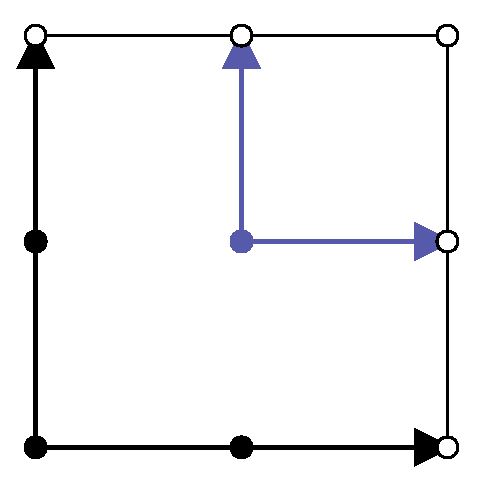
\includegraphics[width=.8\textwidth]{./data/sketches/2_sc.pdf}
	\hfill
	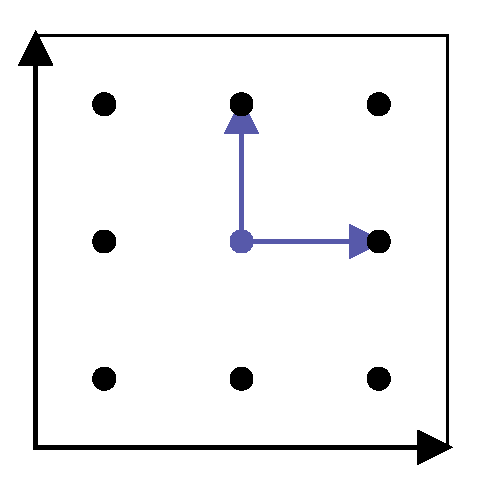
\includegraphics[width=.8\textwidth]{./data/sketches/3_sc.pdf}
	\hfill
	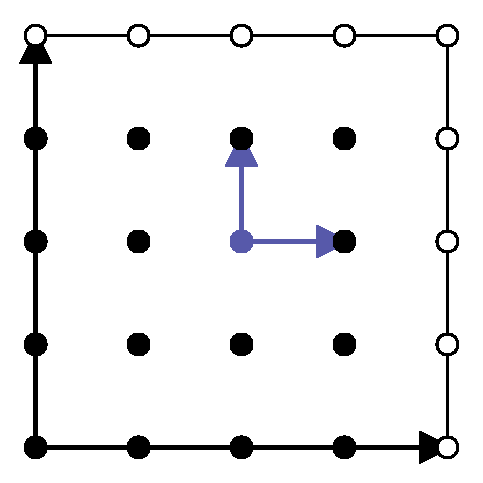
\includegraphics[width=.8\textwidth]{./data/sketches/4_sc.pdf}
	\caption{Depiction of square supercells with lattice points in the range $[-0.5 A, 0.5 A)$ (bullets $\bullet$), and extended lattice points at the supercell boundary (empty bullets $\circ$), where $A$ is the edge length of the supercell. Blue arrows denote the unit cell vectors, black arrows denote the supercell vectors.}
	\label{fig:sketch_supercells}
\end{marginfigure}
These lattice points are included in the Fourier series with an appropriate weight $w_{\b L}$ that accounts for double counting of lattice points that are separated by a linear combination of supercell lattice vectors $\bf S$~\cite{Parlinski.1997}. Furthermore, we use a minimal image convention (MIC) between the atoms $(i, \b 0)$ and $(j, \b L)$: For each pair, we use an equivalent lattice point $\b L'$ within the extended supercell which depends on $(i, j, \b L)$ such that
\begin{align}
	- \b R_{i}^0 + \b R_{j}^0 + \b L' \in \mathds V_{\rm sc}^{\rm ext}~.
	\label{eq:L'}
\end{align}
In total we define
%\marginnote{The dynamical matrix elements defined by Eq.\,\eqref{eq:D_Parlinski} differ from the ones found in Ref.~\cite{Parlinski.1997} by a phase factor ${\rm e}^{\im \b q \cdot (\b R_i^0 - \b R_j^0)}$. The phase factor however does not affect the eigenfrequencies. It typically arises when the discussion is performed from a lattice-wave ansatz to solve the equations of motion~\cite[p. 298]{BornHuang} \TODO{Makes sense to include because harmonic heat flux becomes easier}}
\begin{align}
	{D}_{i \alpha, j \beta} (\tilde{\b q}) 	
		&= %\frac{N}{N_{\rm sc}} 
		\sum_{\b L \in \mathds V_{\rm sc}^{\rm ext}} 
			w_{\b L}
		{\rm e}^{- \im \tilde{\b q} \cdot \b L'} {\rm e}^{\im \tilde{\b q} \cdot (\b R_i^0 - \b R_j^0)} {D}_{i \b 0 \alpha, j \b L \beta}~
	\label{eq:D_Parlinski}
\end{align}
where $\b L'$ is chosen such that it satisfies Eq.\,\eqref{eq:L'}, and the weights $w_{\b L}$ are chosen based on the multiplicity of the lattice point $\b L$ in the extended supercell. The dynamical matrices defined by Eq.\,\eqref{eq:D(q)} and \eqref{eq:D_Parlinski} are equal when evaluated at commensurate $\bf q$-points. We will therefore use the latter definition as \emph{the} dynamical matrix in the following.

\subsection{Properties of the Dynamical Matrix and its Eigenvectors}
\label{sec:dynmat.periodic}
As noted before, the dynamical matrix ${\rm D} (\b q)$ defined in Eq.\,\eqref{eq:D_Parlinski} is a hermitian $3N_{\rm uc} \times 3N_{\rm uc}$ matrix in the indices $(i \alpha, j \beta)$ for each $\b q$ within the Brillouin zone.\footnote{These can be either commensurate points $\bf q$, or interpolated points $\tilde{\bf q}$.} The $3N_{\rm uc}$ eigenvalues will therefore be real, and there will be $3N_{\rm uc}$ complex, orthogonal eigenvectors. In accordance with Eq.\,\eqref{eq:D_IJ} we denote
\begin{subequations}
\label{eq:D_ij(q)}
\begin{align}
	\sum_{j \beta} {D}_{i \alpha, j \beta} (\b q) e_{b, j \beta} (\b q)
		&= \omega^2_b (\b q) \, \fD e_{b, i \alpha} (\b q)~,
	\label{eq:D_ij(q)w} \\
	{D}_{i \alpha, j \beta} (\b q)
		&= \sum_b \omega^2_b (\b q) \, \fD e_{b, i \alpha} (\b q) e^\ast_{b, j \beta} (\b q)~,
\end{align}
\end{subequations}
where the \emph{band index} $b$ is used to discern the $3N_{\rm uc}$ \emph{branches} at each $\b q$.\footnote{The notation highlights that the $\b q$ become quasi-continuous in the $N_{\bf q} \to \infty$ limit. In that case, $\frac{1}{N_{\b q}} \sum_{\b q} \to \int \frac{\d^3 q}{(2 \pi)^3}$} 
Since ${\rm D} (\b q)$ is hermitian, it follows that~\cite{Maradudin.1968}
\begin{align}
	D_{i \alpha, j \beta} (- \b q) 
		& = D_{i \alpha, j \beta}^\ast (\b q)~, \\
	e_{b, i \alpha} (- \b q)
		&= e^\ast_{b, i \alpha} (\b q)~,\text{ and} \\
	\omega_b (- \b q)
		&= \omega_b (\b q)~.
\end{align}
With the help of Eq.\,\eqref{eq:D_ij(q)}, the real-space dynamical matrix $\mathrm D_{IJ}$ for the supercell can be written as
%\footnote{When a supercell is used, the sum is restricted to the commensurate $\b q$ points.}
\begin{align}
%	D_{i \b 0 \alpha, j \b L \beta}
%		& = \frac{1}{N_{\b q}} \sum_{\b q} {\rm e}^{- \im \b q \cdot (\b R_{i}^0 - \b R_{j}^0 - \b L)} {D}_{i \alpha, j \beta} (\b q) \\
%\implies
	D_{i \b L \alpha, j \b K \beta}  
		& = \frac{1}{N_{\b q}} \sum_{\b q} {\rm e}^{- \im \b q \cdot (\b R_{i \b L}^0 - \b R_{j \b K}^0)} {D}_{i \alpha, j \beta} (\b q) \\
		& \equiv  \sum_{b, \b q} \omega_b^2 (\b q) ~ \fD e_{b, i \b L \alpha} (\b q) e^{\ast}_{b, j \b K \beta} (\b q)~.
	\label{eq:D_{iLa}}
\end{align}
The eigenvectors of the $3N_{\rm uc} \times 3N_{\rm uc}$ matrices $\mathrm D (\b q)$ appearing in Eq.\,\eqref{eq:D_ij(q)}, and the eigenvectors of the $3N_{\rm sc} \times 3N_{\rm sc}$ matrix~$D_{IJ}$ appearing in Eq.\,\eqref{eq:D_{iLa}} are related by
\begin{align}
	e_{b, i \b L \alpha} (\b q)
		\equiv \frac{1}{\sqrt{N_{\b q}}} {\rm e}^{- \im \b q  \cdot \b R^0_{i \b L}} \, e_{b, i \alpha} (\b q)~.
\end{align}
%\REM{$e_{b, i \b L \alpha} (\b q)$ are real at \emph{commensurate} q-points, this expresses the 1:1 correspondence between lattice points $\b L$ and reciprocal $\b q$ points.}
The completeness relations accordingly read
\begin{align}
	\sum_{i \b L \alpha} \fD e_{b, i \b L \alpha} (\b q) e^\ast_{b', i \b L \alpha} (\b q') 
		&= \delta_{b b'} \delta (\b q - \b q') \quad \text{and} \quad \\
	\sum_{b, \b q} \fD e_{b, i \b L \alpha} (\b q) e^\ast_{b, j \b K \beta} (\b q)
		&= \delta_{il} \delta_{\b L \b K} \delta_{\alpha \beta}~,
	\label{eq:completeness.e_bq}
\end{align}

\newthought{We use the shorthand notation $s = (b, \b q)$ and $-s = (b, - \b q)$} in the following to simplify the notation, and explicitly refer to the band index $b$ and the wavenumber $\b q$ only when necessary.
With these shorthands, the formulas closely resemble the non-periodic case as introduced in Sec.\,\ref{sec:HA}, with $3N_{\rm sc}$ degrees of freedom, only that the eigenvectors $\b e_{s = (b, \b q)}$ can be complex-valued instead of strictly real. In this notation, the dynamical matrix reads
\begin{align}
D_{I \alpha, J \beta}
&= \sum_s \omega^{2}_{s \vphantom I} \, \fD e_{s, I \alpha} e^\ast_{s, J \beta}~.
\label{eq:D_IJ_s_complex}
\end{align}

%\REM{Group velocities?}
%\REM{Space group symmetries: at least cite Maradadudin.}

\subsection{Phonon dispersions and density of states}
\label{sec:ha.dispersions}

\REM{It makes more sense to discuss the ha. model earlier, i.e., most of what is discussd in ``class. harm. dyn.'' at the end?}

With the dynamical matrix for arbitrary q-points in the Brillouin zone at hand, we are in position to evaluate the spectrum of harmonic vibrational excitations in a crystal,~i.\,e.,~\emph{phonon dispersions} or \emph{phonon band structure}, as well as the \emph{density of states}, often called DOS for short.

The density of states $g (\omega)$ can be used to evaluate Brillouin-zone integrals of functions that depend on the phonon energy $\hbar \omega ({\bf q})$. It is implicitly defined via
\begin{align}
	\braket{f}
		&= \frac{1}{V_{\rm BZ}} \int \frac{\d^3 q}{(2 \pi)^3} ~ f{\boldsymbol (}\omega ({\bf q}) \boldsymbol ) 
		= \int \d \omega ~ f(\omega) g (\omega)~,
\end{align}
where 
\begin{align}
	g(\omega) 
		= \frac{1}{V_{\rm BZ}} \int \frac{\d^3 q}{(2 \pi)^3} \delta \boldsymbol{(}
			\omega ({\bf q}) - \omega
		\boldsymbol{)}~,
	\label{eq:DOS}
\end{align}
The density of states can be computed by evaluating the phonon frequencies $\omega ({\bf q})$ on a grid in the Brillouin zone and use approximations to the $\delta$-function in Eq.\,\eqref{eq:DOS} of finite width, for example by using Gaussian functions, or by using a tetrahedron method where the integration weights on the finite grid are computed analytically based on the dispersion~\cite{Bloechl.1994}.

\newthought{In experiment, dispersions can be probed} by neutron scattering, where the incoming neutron beam scatters inelastically with the phonons in the crystal, and a momentum-dependent scattering amplitude can be measured with peaks corresponding to the phonon frequencies~\cite{Squires}. The phonon spectrum of fcc-silicon compoared to inelastic neutron scattering data is shonw in Fig.\,\ref{fig:ha.dispersion.si}. \begin{figure}
	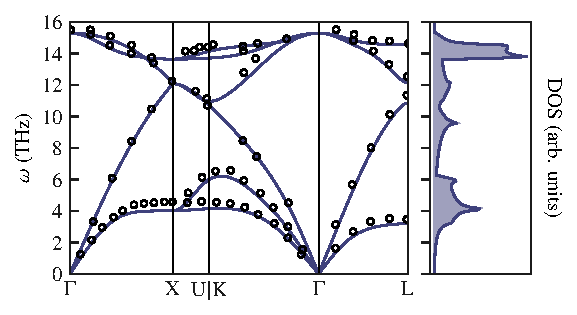
\includegraphics[width=\textwidth]{./data/plots/anharmonicity/3_bandstructures/Si/bands_dos.pdf}
	\caption{
		Phonon bandstructure of fcc-diamond silicon obtained for a supercell with 216 atoms. Open circles denote experimental reference data from inelastic neutron scattering at room temperature~\cite{Nilsson.1972}.
	}
	\label{fig:ha.dispersion.si}
\end{figure}
An alternative approach is \emph{Raman scattering}, where an incoming light beam scatters with a subset of the modes depending on their symmetry properties. Since the light has typical frequencies similar of the vibrational spectrum,~i.\,e., of the order of 10\,THz~$\sim$~40\,meV, its wavenumber $k=\omega/c$ is approximately $3 \cdot 10 ^{-7}$\,\AA$^{-1}$, where $c$ is the speed of light. Taking a typical crystal lattice constant of $a \approx 5\,$\AA, the maximum crystal wavenumber is $q=2 \pi / a \approx 1\,{\text \AA}^{-1}$. Light of similar energy as phonons therefore typically probe the dispersion very close to ${\bf q} = 0$,~i.\,e.,~the $\Gamma$ point. A comparison of calculated phonon dispersion and frequencies from Raman spectroscopy is shown in Fig.\,\ref{fig:ha.dispersion.kcaf3} for the orthorombic perovskite KCaF$_3$~\cite{Bulou.1980, Demetriou.2005, Knight.2005}.
\begin{figure}
	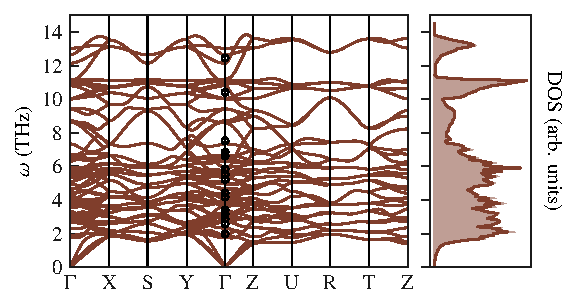
\includegraphics[width=\textwidth]{./data/plots/anharmonicity/3_bandstructures/KCaF3/bands_dos.pdf}
	\caption{
		Phonon bandstructure of KCaF$_3$ in the Pnma structure obtained from a supercell with 160 atoms. Open circles denote experimental reference data from Raman scattering at 40\,K~\cite{Daniel.1997}.
	}
	\label{fig:ha.dispersion.kcaf3}
\end{figure}



\newpage

\section{Statistical Mechanics and Molecular Dynamics}
After discussing nuclear dynamics in the harmonic approximation, and specifying the crystalline state in terms of an intrinsic and extrinsic periodicity in space, we proceed by discussing nuclear dynamics on the full potential energy surface $\mathcal{V} ({\bf R})$ without approximations, but in the classical limes.

\subsection{Classical Limit}
The classical limit of the nuclear Schr\"odinger equation~\eqref{eq:BOSE} is usually performed by writing the nuclear wavefunction $\chi ({\bf R}, t)$ in terms of a real amplitude $A({\bf R}, t)$ and a \emph{classical action function} $S({\bf R}, t)$~\cite{Dirac1981,Landau2013,Marx2009}
\begin{align}
\chi({\bf R}, t) = A({\bf R}, t) \, {\rm e}^{\frac{\im}{\hbar} S({\bf R}, t)}~.
\label{eq:class.1}
\end{align}
The Schr\"odinger equation then yields a set of differential equations for $A$ and $S$ that, in the limit $\hbar \to 0$, go over to a \emph{Hamilton-Jacobi} equation for the action $S$,
\begin{align}
\frac{\partial S}{\partial t} + \mathcal H \left({\bf R}, {\bf P}\right)
= 0~,
\label{eq:HamiltonJacobi}
\end{align}
where ${\bf P} = ({\bf P}_1, \ldots) \equiv ({\bf \nabla}_1 S, \ldots)$ denotes the conjugate momenta and $\mathcal H$ is the \emph{classical} Hamilton function\footnote{We use the terms \emph{Hamilton function} and \emph{Hamiltonian} interchangeably in the following.} corresponding the to the operator in Eq.\,\eqref{eq:BOSE}, from which the equations of motion for the nuclei can be obtained:
\begin{align}
\dot{{\bf P}}_I 
= -\frac{\partial \mathcal H}{\partial {\bf R}_I}
\quad\implies\quad M_I \ddot{\bf R}_I
= -\frac{\partial \mathcal V}{\partial {\bf R}_I}~.
% \equiv - {\bf F}_I~.
\label{eq:dyn.eom.classical}
\end{align}
The negative gradient of the Born-Oppenheimer potential, 
$-\partial \mathcal V / \partial {\bf R}_I$ is the force ${\bf F}_I$ acting on atom $I$ which can be obtained via the Hellmann-Feynman theorem,~cf.~Sec.\,\ref{sec:HellmannFeynman}.

\newthought{An alternative viewpoint} that is more instructive can be taken by invoking the \emph{Ehrenfest theorem}~\cite{Ehrenfest.1927,Basdevant2007}. The statement is that that the time derivative of the expectation value of an atom's momentum ${\bf P}_I$ is given by the expectation value of the negative gradient of the potential,
\begin{align}
\frac{\d}{\d t} \left\langle {\bf P}_I \right\rangle_{\chi}
= \left\langle
- \frac{\partial \mathcal{V}}{\partial {\bf R}_I}
\right\rangle_{\chi}~,
\label{eq:ehrenfest.de1}
\end{align}
where $\langle \cdot \rangle_{\chi}$ denotes an expectation value taken with respect to the nuclear wavefunction $\chi$. This expression differs only slightly from the classical counterpart, which would read
\begin{align}
\frac{\d}{\d t} \left\langle {\bf P}_I \right\rangle
= \left.
- \frac{\partial \mathcal{V}}{\partial {\bf R}_I}
\right\vert_{{\bf R} = \langle {\bf R} \rangle}~.
\label{eq:ehrenfest.de2}
\end{align}
The difference comes from the fact that, in quantum mechanics, the expectation value of a function of an observable does not equal the function of its expectation. In mathematical terms, we have
\begin{align}
\delta f  \equiv 
f \bm ( \langle x \rangle \bm{)} 
- 
\bm{\langle} f (x) \bm{\rangle}
\neq 0
~,
\label{eq:ehrenfest.delta1}
\end{align}
where $x = {\bf R}_I$ denotes the space coordinate, %for notional simplicity, 
$f$ is some function of the observable   $x$, and $\delta f$ measures the difference between the two values,~i.\,e.,~the error introduced by using a classical description. Ehrenfest's argument is that this difference becomes negligible when the state is sufficiently peaked around some value $x_0$. Expanding $f$ around the expectation value of $x$ denoted by $x_0 \equiv \langle x \rangle$, we have
\begin{align}
f(x) = f \bm ( \langle x \rangle \bm{)}  
+ (x - \langle x \rangle) \, f' \bm ( \langle x \rangle \bm{)}
+ \frac{1}{2} (x - \langle x \rangle)^2 \, f'' \bm ( \langle x \rangle \bm{)}
+ \cdots~.
\label{eq:ehrenfest.f2}
\end{align}
It follows that the $f'$ term vanishes when the expectation value is taken, and
\begin{align}
\langle f(x) \rangle 
= f \bm ( \langle x \rangle \bm{)}  
+ \frac{1}{2} \Delta x^2 f'' \bm ( \langle x \rangle \bm{)}
+ \cdots~,
\label{eq:ehrenfest.f3}
\end{align}
where $\Delta x^2 = \bm{\langle} (x - \langle x \rangle)^2 \bm{\rangle}$ measures the variance of the underlying distribution,~i.\,e.~the width of the wavepacket. The relative error between the classical and quantum expectation value is %readily computed to be 
therefore proportional to the variance $\Delta x^2$,
\begin{align}
\left\lvert \frac{\delta f}{f \bm ( \langle x \rangle \bm{)}} \right\rvert
= \frac{1}{2} \Delta x^2 \left\lvert \frac{f'' \bm ( \langle x \rangle \bm{)}}{f \bm ( \langle x \rangle \bm{)}} \right\rvert
+ \mathcal{O}(\Delta x^3)~.
\label{eq:ehrenfest.delta2}
\end{align}
This estimation is general and holds for any observable $f$.
By crudely estimating the dimension of the wavepacket in terms of the thermal de Broglie-wavelength, we find
\begin{align}
\Delta x^2 
\sim \left( \frac{h}{P} \right)^2
\sim \frac{h^2}{MT}~,
\label{eq:ehrenfest:dimension}
\end{align}
where $h$ is Planck's constants, $M$ is the atomic mass, and $T$ is temperature. This estimate gives support to the intuitive assumption that we can expect the classical limit to work better the heavier the atoms and the higher the temperature.
Let us now set $f(x) \hat = -\partial \mathcal V / \partial {\bf R}_I$, then another important conclusion can be drawn from Eq.\,\eqref{eq:ehrenfest.delta2}: For a harmonic potential $\mathcal V ({\bf R}) = \mathcal V^{(2)} ({\bf R})$, where derivatives higher than second order vanish, the classical and quantum mechanical expectation values \emph{coincide}. The quantum mechanical expectation value of the position will therefore evolve in the same time-periodic fashion as a classical particle in a harmonic well.

\newthought{These considerations naturally lead to the formulation of \emph{ab initio} molecular dynamics simulations}, where the time evolution of a system of particles is simulated by propagating the classical equations of motion for each particle on the Born-Oppenheimer potential energy surface, $\mathcal V ({\bf R})$~\cite{Parrinello.1981,Car.1985}. In conjunction with classical statistical mechanics, a wealth of thermodynamic properties of materials can be simulated.
We note in passing that
%Of course, this approach can only be validated by computing observables and comparing the results to experimental . One can safely say that this approach has been used successfully in a plethora of studies, while 
additional care must be taken at low temperatures and for systems with light atoms, especially hydrogen-bonded systems, because in these cases the quantum nature of the nuclei can become non-negligible, as already mentioned in the discussion following Eq.\,\eqref{eq:ehrenfest:dimension}~\cite{Parrinello.1984,Markland.2018,Litman.2020}.

\newthought{As there exist plenty of excellent books on statistical mechanics}, some of which are included in the references~\cite{Phillies2012,Tuckerman,Schrodinger1989}, this chapter mainly serves to recall the most important notions necessary for computing properties of materials under thermodynamic conditions, and introduce the notation used in the remainder of the work. In particular, the concepts of \emph{ensemble}, \emph{state}, and \emph{averages} are briefly introduced.

\subsection{Phase space and ergodic hypothesis}
\label{sec:phase_space}

A thermodynamic \emph{ensemble} can be viewed as a complete list of all allowed \emph{states} $\Gamma$ of a system of particles, where the state is an instantaneous snapshot of all microscopic variables~\cite{Phillies2012}. In classical statistical mechanics, these variables are the $N$ positions~${\bf R} = ({\bf R}_1, \ldots, {\bf R}_{N})$ and momenta~${\bf P} = ({\bf P}_1, \ldots, {\bf P}_{N})$.\footnote{We denote by $N$ either the number of atoms in a system of finite size, or, in periodic systems, the number of atoms in the simulation cell, $N_{\rm sc}$.} A particular configuration $\Gamma = \set{\b R, \b P}$ is called \emph{phase-space point}, and the phase space is the collection of all points $\Gamma$ compliant with external constraints.\footnote{The simplext example of an external constraint: If the particles are confined in a box with impenetrable walls, the possible position $\b R$ are necessarily confined to that box. Other constraints comprise total energy, particle number, and more.} To each state $\Gamma$, a statistical weight $f (\Gamma)$ is assigned, where $f$ is called the \emph{distribution function}. A thermodynamic ensemble is completely specified by the set of external constraints under which the mechanical system evolves, and the associated statistical weight function $f$.

\newthought{Statistical averages of phase-space functions} can be obtained by averaging over all permissible states $\Gamma$ with the statistical weight given by the distribution function, $f (\Gamma)$. The \emph{phase-space average} of a generic phase-space function $A (\Gamma)$ is defined as
\begin{align}
  \braket{A}_f 
    = \int \d \Gamma ~ A(\Gamma) f (\Gamma)~.
  \label{eq:phase.space.average}
\end{align}

An alternative approach towards computing averages is the concept of time averaging. The \emph{time average} of a phase-space function is defined as
\begin{align}
  \braket{A}_t
    = \lim\limits_{t \to \infty} \frac{1}{t} \int_0^t \d t' ~ A {\bm (} \Gamma_{t'} {\bm )}~,
  \label{eq:time.average}
\end{align}
where $\Gamma_t = \set{ {\bf R} (t), {\bf P} (t)}$ denotes a phase-space point at time $t$ after evolving from an initial point $\Gamma_0$ as explained in the next section.
A system for which the phase-space and the time average are identical is said to be \emph{ergodic}. The \emph{ergodic hypothesis} states that this is true for most systems with non-pathological particle interaction $\mathcal V$. Albeit being virtually impossible to prove rigorously, this hypothesis is the underlying idea of \emph{molecular dynamics} (MD) simulations, where the statistical behavior of a system is assessed by choosing a suitable initial condition and propagating it in time by numerically solving the equations of motion.

\newthought{In this work}, we use two thermodynamic ensembles: the microcanonical, $NVE$ for short, where the total energy $E$ of the system is conserved, and the canonical ($NVT$), where the system can be viewed as coupled to a bath of temperature $T$. The latter is mimicking more realistic experimental conditions, where usually the temperature and not the total energy of the system can be controlled. Technically, experiments are performed rather at constants pressure $p$ instead of constant volume, and the correct ensemble to describe such a situation is the isothermal-isobaric one commonly denoted as $NPT$. In practice however, the canonical ensemble is easier to simulate and is a good approximation to the $NPT$ ensemble when the system size is not too small~\cite[p.\,134]{Tuckerman}


\subsection{Microcanonical Ensemble}
The microcanonical ensemble is characterized by three conserved extensive quantities: particle number $N$, system volume $V$, and total energy $E$. The total energy of a given microstate,~i.\,e.,~the configuration of particles and their momenta represented by the phase-space point $\Gamma = \set{\b R, \b P}$, is given by the Hamiltonian of the system, $\mathcal H (\Gamma)$. 
%The central postulate of statistical mechanics is that each microstate is equally probable. Therefore, any point in phase space $\Gamma$ yielding an energy in a thin interval around the target energy, $H (\Gamma) \in [E, E + \d E]$, is realized with the same likelihood. Taking particle number $N$ and system volume $V$ to be fixed and non-controllable, the expectation value of a phase-space observable $A$ in an ensemble of energy $E$ is defined as
%\begin{align}
%	\braket{A}_E 
%		= \int \d \Gamma ~ A(\Gamma) f_E (\Gamma)~.
%	\label{eq:phase.space.expectation}
%\end{align}
%Here, the \emph{microcanonical distribution function} $f_E$ is enforcing that phase-space points are sampled with equal probability which is achieved by defining
% \newthought{The microcanonical distribution function} is defined as
The microcanonical distribution function is defined as
\begin{align}
f_E (\Gamma) = \frac{1}{\mathcal{Z}_E} \delta {\bm (} \mathcal H (\Gamma) - E {\bm )}~,
\end{align}
where the microcanonical partition function $\mathcal{Z}_E$ is a normalizing factor for $f_E$. The distribution function $f_E$ encapsulates the underlying postulate of the microcanonical ensemble,~i.\,e.,~that any point in phase space $\Gamma$ yielding an energy $\mathcal H (\Gamma)$ in a thin interval around the target energy $E$ 
%, $H (\Gamma) \in [E, E + \d E]$, 
will be realized with the same likelihood.

\newthought{The time evolution of a system} is governed by the Hamiltonian $\mathcal H$ which generates an energy conserving propagation of a phase space point $\Gamma_t = \set{\b R (t), \b P (t)}$ in terms of Hamilton's equations,
\begin{align}
	\dot{\b R}_I (t) = \frac{\partial \mathcal H (t)}{\partial \b P_I} \quad\text{and}\quad
	\dot{\b P}_I (t) = -\frac{\partial \mathcal H (t)}{\partial \b R_I}~.
	\label{eq:stat.eom}
\end{align}
The temporal evolution of a phase-space observable $B (\Gamma_t) \equiv B(t)$ is then given by the Liouville equation~\cite{Tuckerman}
\begin{align}
	\dot{B} (t) = \set{B (t), \mathcal H (t)} \equiv \im \mathcal L B (t)~,
	\label{eq:Liouville}
\end{align}
where $\mathcal L$ is the \emph{Liouville operator} defined by its action according to Eq.\,\eqref{eq:Liouville}, and $\set{\cdot , \cdot}$ denotes the \emph{Poisson bracket}.\marginnote{
The Poisson bracket is defined by
\begin{align}
	\set{B, \mathcal H}
		= \sum_{I, \alpha} \frac{\partial B}{\partial R_I^\alpha} \frac{\partial \mathcal H}{\partial P_I^\alpha}
			- \frac{\partial B}{\partial P_I^\alpha} \frac{\partial \mathcal H}{\partial R_I^\alpha}
%		= \sum_{I, \alpha} \frac{\partial B}{\partial R_I^\alpha} \dot{R}_I^\alpha
%			+ \frac{\partial B}{\partial P_I^\alpha} \dot{P}_I^\alpha~.
	\label{eq:Poisson}
\end{align}
}
The Liouville equation is formally solved by
\begin{align}
	B (t) = {\rm e}^{\im \mathcal L t} B(0)~,
	\label{eq:B.time.evolution}
\end{align}
the operator ${\rm e}^{\im \mathcal L t}$ is therefore called the \emph{time evolution operator} or \emph{classical propagator}.
%\paragraph{Ergodic hypothesis}
%Under the assumption that a system initially prepared in a configuration with correct energy dynamically evolves through the entire permissible phase space, the phase-space average defined in Eq.\,\eqref{eq:phase.space.expectation} can be written in terms of a \emph{time average} defined as
%\begin{align}
%  \braket{A}_E 
%    = \left. \lim\limits_{t \to \infty} \frac{1}{t} \int_0^t \d t' ~ A {\bm (} \Gamma(t') {\bm )}
%	    \right\vert_{H \bm ( \Gamma (0) \bm ) = E}~.
%	\label{eq:time.average}
%\end{align}
%A system for which the phase-space and the time average are identical is said to be \emph{ergodic}. The \emph{ergodic hypothesis} states that this is true for most systems with non-pathological interaction $V$. Albeit being virtually impossible to prove rigorously, this hypothesis is underlying idea of \emph{molecular dynamics} (MD) simulations, where the statistical behavior of a system is assessed by choosing a suitable initial condition and propagating it in time via the classical equations of motion given by Eq.\,\eqref{eq:stat.eom}.
In practice, the equations of motion are solved numerically, for example by the \emph{velocity Verlet} algorithm~\cite{Verlet.1967},
\begin{subequations}
\begin{align}
	\b R_I (t + \delta t) 
		&= \b R_I (t) + \delta t \dot{\b R}_I (t) + \frac{\delta t^2}{2 M_I} \b F_I(t) + \mathcal{O} (\delta t^4)~, \\
	\dot{\b R}_I (t + \delta t) 
		&= \dot{\b R}_I (t) + \frac{\delta t}{2 M_I} \left[\b F_I(t) + \b F_I (t + \delta t)\right] + \mathcal{O} (\delta t^4)~.
\end{align}
\label{eq:VelocityVerlet}
\end{subequations}
The velocity Verlet algorithm introduces an error of order $\delta t^4$ in the integration step, but has two important properties mitigating a negative impact on obervables: First, a velocity Verlet integration step is time-reversible, an important prerequisite for long-term stability of the total energy for symmetry reasons. Second, the velocity Verlet map from $t$ to $t + \delta t$ has the property of being \emph{symplectic}~\cite[p.\,101]{Tuckerman}. This means that the discrete time propagation is not guaranteed to preserve the energy along the trajectory $\Gamma_t$, but there exists a Hamiltonian $\tilde{\mathcal H} (\Gamma, \delta t)$ which is conserved exactly and fulfills $\tilde{\mathcal H (\Gamma, \delta t)} \to \mathcal H(\Gamma)$ for vanishing timestep $\delta t \to 0$~\cite[p.\,121]{Tuckerman}. The symplectic property is formalized in the ``shadowing theorem'', which states that existence of a ``shadow Hamiltonian'' $\tilde{\mathcal H}$ ensures that errors introduced by using a finite time step are bounded~\cite[p.
,120]{Tuckerman}.

\subsection{Canonical ensemble}
The canonical ensemble is characterized by the two extensive variables particle number $N$ and volume $V$, and the intensive quantity temperature $T$. It can be viewed as representing a system in contact with an infinite thermal bath of temperature $T$, where heat can be exchanged via a weak coupling.

In analogy to the previous section, the \emph{canonical distribution function} at inverse temperature $\beta = 1 / k_{\rm B} T$ is defined as
%
\begin{align}
	f_\beta (\Gamma) 
		= \frac{1}{\mathcal{Z}_\beta} {\rm e}^{- \beta \mathcal H (\Gamma)}~,
	\label{eq:f.canonical}
\end{align}
%
where the  canonical partition sum $\mathcal{Z}_\beta$ normalizes $f_\beta$. 
%The canonical expectation value is therefore given by
%\begin{align}
%	\braket{A}_\beta = \int \d \Gamma ~ A(\Gamma) f_\beta(\Gamma)~.
%\end{align}

\newthought{As we have seen earlier}, a time-independent Hamiltonian generates energy-preserving dynamics via the equations of motion given in Eq.\,\eqref{eq:stat.eom}. To perform a simulation at non-constant energy, the coupling to a thermal bath therefore has to be incorporated explicitly into the equations of motion. One of the many ways to achieve this is via the \emph{Langevin equation}~\cite{Vanden.2006} in which the change of momentum is modified,
\begin{align}
	\dot{\b P}_I (t) 
		&= \b F_I (t) - \gamma \b P_I (t) + \b F^{\rm stochastic}_I (t)~.
	\label{eq:stat.Langevin}
\end{align}
This equation describes a perturbation of the nuclei induced by a velocity-dependent friction proportional to a constant $\gamma$, %\marginnote{From Eq.\,\eqref{eq:stat.Langevin} follows that $\gamma$ has the unit of inverse time.}
and a stochastic force proportional to a white-noise kernel $\eta (t)$.\footnote{
	% \normalsize
	The stochastic force is given by:
	\begin{align*}
	\b F^{\rm stochastic}_I (t) 
	&= \sqrt{2 k_{\rm B} T M_I \gamma} \eta (t)~, \\
	\braket{\eta (t) \eta (0)}
	& = \delta (t)~.
	\end{align*}
	It replenishes the kinetic energy dissipated by the friction proportinoal to $\gamma$, see discussion in Ref.\,\cite[p.\,328]{Phillies2012}.
}
With the modified equations of motion in terms of the stochastic force, an ergodic time evolution that generates the canonical distribution can be obtained, so that
\begin{align}
  \braket{A}_t = \braket{A}_{T}~.
\end{align}
%hypothesis for the canonical ensemble can be stated,
%% 
%\begin{align}
%	\braket{A}_\beta
%		= \left. \lim\limits_{t \to \infty} \frac{1}{t} \int_0^t \d t' ~ A {\bm (} \Gamma(t') {\bm )}
%			\right.~,
%	\label{eq:time.average.canonical}
%\end{align}
%where the time evolution of the system is given by Eq.\,\eqref{eq:stat.Langevin} and the friction constant is chosen such that the expectation value $\braket{A}_\beta$ is insensitive to the chosen value.
In practice, the Langevin equation can be used to thermalize a system and generate a canonical ensemble starting from some initial configuration $\b R^0$~\cite[p.\,590]{Tuckerman}.

Other ways of generating an $NVT$ ensemble are deterministic Nos\'e-Hoover simulations, or the stochastic velocity rescaling approach that can preserve spectral properties~\cite{Nose.1984,Hoover.1985,Bussi.2007}.

%\REM{Maxwell-Boltzmann distribution}
%
%\REM{Plot of thermalization period}

\newpage

\section{Classical harmonic dynamics and harmonic mapping}
Also the harmonic Hamiltonian defined in Eq.\,\eqref{eq:ha.H2} generates classical dynamics by means of the canonical equations of motion for the normal coordinates $\set{ u_s, p_s}$,\footnote{We deal with the finite simulation cell, where the dynamical matrix is a symmetric matrix with real eigenvalues $\omega^2_s$ and real eigenvectors ${\bf e}_{sI}$.}
\begin{align}
\dot{u}_s
& = \frac{\partial \mathcal H^{(2)}}{\partial p_s}
= p_s~,\quad\text{and}\quad
\dot{p}_s
= - \frac{\partial \mathcal H^{(2)}}{\partial u_s}
= - \omega^2_s u_s~.
\label{eq:ha.canonical.eom}
\end{align}
These equations of motion can be solved in straightforward fashion in terms of plane waves for the normal mode coordinates $\set{u_s, p_s}$. We find it, however, more instructive to find a solution in formal similarity with quantum mechanics,\footnote{The relation to quantum mechanics is achieved by replacing the complex numbers $a_s$ with the operators $\hat{a}_s$ fulfilling the canonical commutation relations $$\left[ \fD{\hat{a}}_{\fP s}, \D{\hat a}_{s'} \right] = \delta_{ss'}~.$$} by first expressing the real normal coordinates $\set{u_s, p_s}$ terms of complex, unitless amplitudes $\set{a_s}$ as
\begin{subequations}
	\label{eq:u_s.amplitudes}
	\begin{align}
	u_s (t) 
	&\equiv ~ \sqrt{\frac{\hbar}{2 \omega_s}} \left[ \D a_s (t) + \fD a_s (t) \right]~, \\
	p_s (t) 
	&\equiv \im \sqrt{\frac{\hbar \omega_s}{2}} \left[ \D a_s (t) - \fD a_s (t) \right]~,
	\end{align}
\end{subequations}
with the inverse relation
\begin{align}
	a_s
	&= \sqrt{\frac{\omega_s}{2 \hbar}} u_s + \frac{\im}{\sqrt{2 \hbar \omega_s}} p_s 	\label{eq:a_st}~,
\end{align}
where $\D a_s$ denotes the complex conjugate of $a_s$. 
In terms of these amplitudes, the harmonic Hamiltonian reads
\begin{align}
	\mathcal{H}^{(2)} (\b a, t)
		&= \sum_s \hbar \omega_s \D a_s (t) \fD a_s (t)
	\equiv \sum_s \hbar \omega_s n_s (t)~,
	\label{eq:Hamiltonian.aa}
\end{align}
where we identify the squared modulus of the amplitudes with the \emph{mode occupation} $n_s$,
\begin{align}
	\D a_s (t) \fD a_s (t) \equiv n_s (t)~.
	\label{eq:ha.occ}
\end{align}
The time derivative of the amplitude $a_s$ is found by using the classical equations of motions given in Eq.\,\eqref{eq:ha.canonical.eom},
\begin{align}
	\dot a_s
		% &= \sqrt{\frac{\omega_s}{2 \hbar}} \dot u_s + \frac{\im}{\sqrt{2 \hbar \omega_s}} \dot p_s
		= - \im \omega_s a_s~,
	\label{eq:dot_a_s}
\end{align}
so that $a_s (t)$ is given in terms of a complex plane wave,
	\begin{align}
		a_s (t) 
			& = {\rm e}^{- \im \omega_s t} a_s (0)~.
			\label{eq:a_s(t)}
%		a_s (0)
%			& = \sqrt{n_s} {\rm e}^{- \im \varphi_s}~,
	\end{align}
It is evident that in the purely harmonic dynamics, the mode occupation defined in Eq.\,\eqref{eq:ha.occ} is constant in time, $n_s (t) \equiv n_s = {\rm const}$. We therefore express the amplitudes at intial time $t=0$ as
\begin{align}
	a_s (0)
		& = \sqrt{n_s} {\rm e}^{- \im \varphi_s}~,
\end{align}
where $n_s$ and $\varphi_s$ are chosen based on the initial configuration of atoms.


By using this solution for the normal coordinates $\set{u_s, p_s}$ in Eq.\,\eqref{eq:u_s.amplitudes}, we find
\begin{subequations}
	\label{eq:u_p_st}
	\begin{align}
	u_s (t) 
	&= \phantom{\omega_s} A_s \sin (\omega_s t + \varphi_s)~,
	\label{eq:u_s(t)}
	\\
	p_s (t) 
	&= \omega_s A_s \cos (\omega_s t + \varphi_s)~,
	\end{align}
\end{subequations}
where 
\begin{align}
	A_s = \sqrt{\frac{2 \hbar n_s}{\omega_s}}
\end{align}
is the amplitude of the mode displacement $u_s$.

\newthought{For a system in thermal equilibrium at a finite temperature $T$}, the mode occupation $n_s$ can be estimated
by analogy with quantum mechanics, where the harmonic energy is given by~\cite{Dove}
\begin{align}
	\braket{\mathcal H^{(2)}}_T
		=\sum_{s} \hbar \omega_{s}\left(n_{\mathrm{B}}\left(\omega_{s}, T\right)+\frac{1}{2}\right)~,
\end{align}
with the Bose function $n_{\rm B} (\omega, T)$ giving the occupation of state of energy $\hbar \omega$ at temperature $T$.\footnote{Bose function ($\beta = 1 / k_{\mathrm{B}} T$): $$n_{\mathrm{B}}(\omega, T)=\frac{1}{\mathrm{e}^{\, \beta \hbar \omega}-1}~.$$}
The expectation of the mode amplitude is therefore given by
\begin{align}
	\braket{n_s}_T
		= \left(n_{\mathrm{B}}(\omega_s, T)+\frac{1}{2}\right)
	\quad\underset{k_{\rm B} T \gg \hbar \omega_s}{\longrightarrow}\quad
	\frac{k_{\rm B} T}{\hbar \omega_s}~,
	\label{eq:ha.amplitude.expectation}
\end{align}
i.\,e., in the high temperature limit, the energy of the mode $s$ given by \mbox{$E_s = \hbar \omega_s \braket{n_s}_T$} approaches the \emph{equipartition} value
\begin{align}
	E_s = k_{\rm B} T~.
	\label{eq:E.equipartition}
\end{align}

\subsection{Harmonic sampling}
\label{sec:harmonic_sampling}
The solution to the equations of motion for the normal coordinates given in Eq.\,\eqref{eq:u_p_st} can be used to describe the time evolution of the real-space displacements ${\bf U}_I (t)$,
\begin{align}
	{\bf U}_I (t) 
		&= \frac{1}{\sqrt{M_I}} {\bf u}_I (t) 
		= \frac{1}{\sqrt{M_I}} \sum_s {\bf e}_{sI} u_s (t) \\
		&= \frac{1}{\sqrt{M_I}} \sum_s  A_s \b e_{sI} \sin (\omega_s t + \varphi_s)~,
\end{align}
where ${\bf e}_{sI}$ denotes the eigenvector elements corresponding to mode $s$ and atom $I$. This equation can be used to generate atomic configurations representative for a given temperature via
\begin{align}
	{\bf U}_I = \frac{1}{\sqrt{M_I}} \sum_s  \zeta_s \braket{A_s}_T \b e_{sI}~,
	\label{eq:ha.samples}
\end{align}
where $\braket{A_s}_T = \sqrt{\frac{2 \hbar \braket{n_s}_T}{\omega_s}}$ is the mean mode amplitude in terms of the mean mode occupation $\braket{n_s}_T$ given by Eq.\,\eqref{eq:ha.amplitude.expectation}, and $\zeta_s$ is a normally distributed random number mimicking thermal fluctuations~\cite{West.2006}. The practical use of Eq.\,\eqref{eq:ha.samples} is twofold: First, it can be used to pre-thermalize molecular dynamics simulations by providing a approximately correct distribution of displacements. Second, it can be used to estimate thermodynamic expectation values of configuration-dependent observables by approximating the ensemble average with respect to the full potential $\mathcal V ({\bf R})$,
\begin{align}
	\braket{B ({\bf R})}_T
		= \frac{1}{\mathcal{Z}_{\mathcal{V}}} \int \d {\bf R} \,{\rm e}^{- \beta \mathcal V ({\bf R})} B({\bf R})~,
	\label{eq:ha.expectation.0}
\end{align}
with an average with respect to the harmonic potential,
\begin{align}
	\braket{B ({\bf R})}_T^{(2)}
		= \frac{1}{\mathcal{Z}_{\mathcal{V}^{(2)}}} \int \d {\bf R} \,{\rm e}^{- \beta \mathcal V^{(2)} ({\bf R})} B({\bf R})
		\approx  \frac{1}{M} \sum\limits_{m=1}^{M} B({\bf R}_m)~,
\label{eq:ha.expectation.1}
\end{align}
where ${\bf R}_m$ denotes a sample generated by Eq.\,\eqref{eq:ha.samples}, and $M$ ist the total number of samples~\cite[p.\,15]{FrenkelSmit}. This sampling approach can be understood as a harmonic Monte Carlo approach~\cite{West.2006,Peslherbe.1999}.
%\mscomment{this is not textbook, explain more}
%\FK{I think it's textbook.}

\subsection{Harmonic mapping}
In the previous section, we have investigated the time evolution of (mode) displacements generated by the harmonic model in analytical fashion. We found that the mode occupations $n_s$, and therefore the energy of each mode, $E_s$, were constant in time. Pictorially, this can be explained by the absence of interactions between the normal modes -- once a mode is excited, it cannot lose or gain energy.
The interaction of vibrational modes can be computed by means of perturbation theory,~i.\,e.,~by computing the transition amplitudes between modes when taking higher than second-order force constants into account, or by using molecular dynamics simulations, where the interactions are naturally described non-perturbatively. All effects not described by the harmonic model are therefore called \emph{anharmonic}, and we will investigate this topic in more detail in chapter~\ref{chp:anharmonicity}. 
Since the normal mode displacements and momenta $\set{u_s, p_s}$ are obtained by means of a unitary transformation from the atom positions and momenta, $\set{{\bf R}_I, {\bf P}_I}$, they provide a complete basis in which the nuclear dynamics can be described, even when anharmonic effects are considered. When anharmonic effects are not too strong, the main effect of interactions are a shift in frequencies, and finite lifetimes.

\newthought{In order to map the dynamical evolution of the system onto the normal modes}, we recall that normal mode coordinates an real-space coordinates are related by the eigenvectors ${\bf e}_{sI}$ of the dynamical matrix,~i.\,e.,
%
\begin{subequations}
	\label{eq:u_p_st.real}
\begin{align}
u_s (t)
&= \sum_{I} {\bf e}_{s, I} \cdot {\bf u}_{I} (t)
~,\quad\text{and}
\label{eq:u_st.real)} \\
p_s (t)
&=\sum_{I} {\bf e}_{s, I} \cdot {\bf p}_{I} (t) ~,
\label{eq:p_st.real}
\end{align}
\end{subequations}
%
from which the time-dependent complex amplitude $a_s (t)$ can be found by means of Eq.\,\eqref{eq:a_st},~i.\,e.,
\begin{align}
		a_s (t)
		&= \sqrt{\frac{\omega_s}{2 \hbar}} u_s (t) + \frac{\im}{\sqrt{2 \hbar \omega_s}} p_s (t)~,
\end{align}
with $\set{u_s (t), p_s (t)}$ given in terms of the real-space dynamics by Eq.\,\eqref{eq:u_p_st.real}. In terms of this complex amplitude, the mode occupation $n_s$ becomes time-dependent,
\begin{align}
	n_s (t) = \D a_s (t) \fD a_s (t)~,
	\label{eq:n_s(t)}
\end{align}
as well as the mode energy,
\begin{align}
	E_s (t) = \hbar \omega_s n_s (t)~.
\end{align}
We will later see how the time-dependent, mode-resolved energy can be used to extract phonon lifetimes from molecular dynamics simulations.
%\REM{Move this discussion to here?}

\newthought{As a final remark}, we like to point out that for periodic systems, where $s=(b, {\bf q})$, the eigenvectors used in the transformation defined in Eq.\,\eqref{eq:u_p_st.real} are not strictly real, and therefore the normal mode coordiantes $\set{u_s, p_s}$ can be complex numbers already. In this situation, one needs to define two independent complex amplitudes, $a_s$ and $a_{-s}$, where $s = (b, - {\bf q})$ denotes a mode with opposite wave vector~\cite[p.\,300]{BornHuang}. In this case, we define\footnote{The explicit formulas in terms of $(b, {\bf q})$ are given in appendix~\ref{app:formulas.ha}.}
%
\begin{subequations}
	\label{eq:u_s.periodic}
\begin{align}
u_s (t)
&= \sum_{I} {\bf e}_{s, I} \cdot {\bf u}_{I} (t)~,
\label{eq:u_st)} \\
p_s (t)
&=\sum_{I} {\bf e}_{s, I} \cdot {\bf p}_{I} (t) ~.
\label{eq:p_st.periodic}
\end{align}
\end{subequations}
%
%\TODO{check conjugation w.r.t. to BornHuang Eq. 38.26/27}
%
with
\begin{subequations}
	\label{eq:u_s.amplitudes.periodic}
	\begin{align}
	u_s (t) 
	&\equiv \frac{1}{\sqrt{2 \omega_{s}}} \left[ \D a_{-s} (t) + \fD a_s (t) \right]~, \\
	p_s (t) 
	&\equiv \im \sqrt{\frac{\omega_s}{2}} \left[ \D a_{-s} (t) - \fD a_s (t) \right]~,
	\end{align}
\end{subequations}
and the corresponding inverse relations
\begin{subequations}
	\label{eq:a(q)}
	\begin{align}
	a_s
	&= \sqrt{\frac{\omega_s}{2}} u_s + \frac{\im}{\sqrt{2 \omega_s}} p_s \\
	a^\dagger_{-s}
	&= \sqrt{\frac{\omega_s}{2}} u_s - \frac{\im}{\sqrt{2 \omega_s}} p_s~,
	\end{align}
\end{subequations}
in units where $\hbar = 1$. Using these amplitudes, the harmonic Hamiltonian reads
\begin{align}
	\mathcal{H}^{(2)}
		&= \halb \sum_s \omega_s \left( \D a_s \fD a_s + \D a_{-s} \fD a_{-s} \right) \\
		&= \sum_s \omega_s \D a_s \fD a_s
\end{align}
where the last line holds when the summation contains both $\bf q$ and $- {\bf q}$, because $\omega_s = \omega_{-s}$.

%\mscomment{shorten and cite textbooks}
%\FK{\cite{BornHuang,Maradudin}}

%\REM{Only real case?}
%
%In the finite simulation box, ${\rm D}_{IJ}$ is symmetric matrix with real eigenvalues and eigenvectors
%
%\begin{align}
%\mathcal{H}^{(2)}(t)
%&= \halb \sum_I {\bf p}_I^2 (t) + 
%\halb \sum_{\substack{I, J \\ \alpha, \beta}}
%D_{I \alpha, J \beta}
%\, u_I^\alpha (t) u_J^\beta (t)~.
%\end{align}
%
%diagonalize by Eq.\,\eqref{eq:D_IJ}
%
%\begin{align}
%\mathcal{H}^{(2)}(t)
%&= \halb \sum_s p_s (t)^2 + 
%\halb \sum_{s} \omega_s^2	\, u_s (t))^2~,
%\label{eq:ha.H2.complex}
%\end{align}
%
%where now the mode displacements $u_s$ and momenta $p_s$ are given by 
%
%
%
%
%Before concluding the chapter, we discuss classical harmonic dynamics. We recall the harmonic Hamiltonian initially defined in Eq.\,\eqref{eq:ha.H2}
%\begin{align}
%\mathcal{H}^{(2)}(t)
%&= \halb \sum_s |p_s (t)|^2 + 
%\halb \sum_{s} \omega_s^2	\, |u_s (t))|^2~,
%\label{eq:ha.H2.complex}
%\end{align}
%
%
%
%\begin{align}
%\mathcal{H}^{(2)}(t)
%	&= \halb \sum_s |p_s (t)|^2 + 
%	\halb \sum_{s} \omega_s^2	\, |u_s (t))|^2~,
%	\label{eq:ha.H2.complex}
%\end{align}
%
%
%
%
%\begin{align}
%\b u_I (t) 
%&= ~\sum_s \frac{1}{\sqrt{2 \omega_s}} \b e^\ast_{s I} \left[ \D a_{-s} (t) + \fD a_s (t)\right]~,\quad\text{and} \\
%\b p_I (t) 
%&= \sum_s ~\im \sqrt{\frac{\omega_s}{2}} ~ {\b e}_{s I} \left[ \D a_{-s} (t) - \fD a_s (t) \right]~,
%\end{align}
%
%with the slight modification that, in the periodic case, the mode displacements $u_s$ and momenta $p_s$ can be complex.
%
%
%
%
%%\begin{align}
%%u_b (\b q, t) 
%%& = \sum_{i \b L} \sqrt{M_I} \, \b e_{s, i\b L} (\b q) \cdot \b U_{i \b L} (t) ~,
%%\label{eq:mode.projection.u_b(q)}
%%\end{align}
%%and likewise for $p_b (\b q, t)$ with $\set{\dot{\b U}_{i \b L}}$ instead of $\set{\b U_{i \b L}}$.
%%
%%\subsection{Classical harmonic dynamics}
%
%
%
%\subsection{Mode projection}
%
%Express amplitude $a_s (t)$ in terms of the atomic displacements $\set{\b U_I (t)}$ and velocities $\set{\dot{\b U}_I (t)}$ \TODO{Check units!}
%The inverse relation between the amplitudes $a_s$ in terms of the conjugate variables $\set{u_s, p_s}$ is
%\begin{align}
%a_s (t) = \sqrt{\frac{\omega_s}{2}} u_s (t) + \frac{\im}{\sqrt{2 \omega_s}} p_s (t)
%\end{align}
%with
%\begin{subequations}
%	\label{eq:mode.projection.u_s}
%	\begin{align}
%	u_s (t) 
%	& = \sum_I \sqrt{M_I} \b e_{sI} \cdot \b U_I (t) ~,
%	%\\
%	%	p_s (t)
%	%	    & = \sum_I \sqrt{M_I} \b e_{sI} \cdot \dot{\b U}_I (t) %\\
%	%	\implies
%	%	a_s (t) 
%	%	    &= \sum_I \sqrt{M_I} \b e_{sI} \cdot \left[ \b U_I(t) + \frac{\im}{\omega_s} \dot{\b U}_I (t) \right]
%	\end{align}
%\end{subequations}
%and likewise for $p_s (t)$ with $\set{\dot{\b U}_I}$ instead of $\set{\b U_I}$.
%
%
%In terms of complex amplitudes $a^{(\dagger)}_s$, we define
%%\marginnote{The sign convention enforces that $$u_b^\ast (\b q) = u_b (- \b q)~,$$ so that the displacements $u_I$ are always real.}
%\begin{subequations}
%	\label{eq:u_s.amplitudes.periodic}
%	\begin{align}
%	u_s (t) 
%	&\equiv \frac{1}{\sqrt{2 \omega_{s}}} \left[ \D a_{-s} (t) + \fD a_s (t) \right]~, \\
%	p_s (t) 
%	&\equiv \im \sqrt{\frac{\omega_s}{2}} \left[ \D a_{-s} (t) - \fD a_s (t) \right]~,
%	\end{align}
%\end{subequations}
%The inverse relations are given by
%\begin{subequations}
%	\label{eq:a(q)}
%	\begin{align}
%	a_s
%	&= \sqrt{\frac{\omega_s}{2}} u_s + \frac{\im}{\sqrt{2 \omega_s}} p_s \\
%	a^\dagger_{-s}
%	&= \sqrt{\frac{\omega_s}{2}} u_s - \frac{\im}{\sqrt{2 \omega_s}} p_s
%	\end{align}
%\end{subequations}
%The displacements are recovered by
%\begin{align}
%\b u_{i \b L}
%&= \frac{1}{\sqrt{N_{\b q}}} \sum_{s} {\rm e}^{\im  \b q \cdot \b R^0_{i \b L}} \, \b e^\ast_{s i} \fD u_s
%\label{eq:u_iL}
%\end{align}
%%\end{subequations}
%and likewise for $\b p_{i \b L}$.
%
%\newthought{By using the property $\omega_s = \omega_{\-s}$}, the Hamiltonian can be brought into the form given earlier in Eq.\,\eqref{eq:Hamiltonian.aa}, and the time evolution of the operators is given by Eq.\,\eqref{eq:a_s(t)}.